
\section{Support Vector Machine}

Les \og{}Support Vector Machine\fg{} ou machines à vecteur de support sont un
ensemble de techniques d'apprentissage supervisé efficace dans les tache de
classification. Historiquement, ils ont été développés dans les années 1990 à
partir des considérations théoriques de Vladimir Vapnik surle développement
d'une théorie statistique de l'apprentissage: la théorie de
Vapnik-Tchervonenkis. L’idée est de rechercher une règle de décision basée 
sur une séparation par hyperplan de marge optimale.

\subsection{Quelques définitions}

\subsubsection{Hyperplan}
Dans un espace vectoriel de dimension finie $n$, un hyperplan est un
sous-espace vectoriel de dimension $n−1$. Ainsi, dans un espace de dimension
$2$ un hyperplan sera une droite, dans un espace de dimension $3$ un hyperplan
sera un plan, etc.
L’équation caractéristique d’un hyperplan est de la forme
\[w_1x_1+w_2x_2+\dots+w_nx_n=0\] où $w_1, w_2, \cdots, w_n$ sont des scalaires.
Un hyperplan sépare complètement l'espace vectoriel en deux parties distinces.
Cette théorie est utilisé en apprentissage automatique dans le but de classer
distinctement un ensemble de données étiquettés.  Les paramètres qui régissent
l'équation permettant d'y arriver sont alors les variables à apprendre
(caractéristiques).

\begin{figure}[h!]
\begin{center}
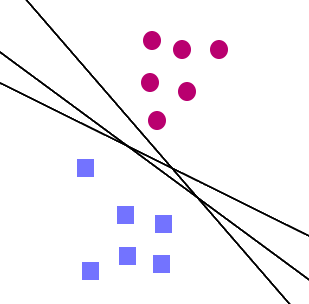
\includegraphics[width=14cm]
{images/hyperplan.png}
\caption{Hyperplan.\label{fig:hyperplan}}
\end{center}
\end{figure}

\subsubsection{Marge}
La marge est la distance minimale de l’hyperplan à un des points d’entraînement.

\begin{figure}[h!]
\begin{center}
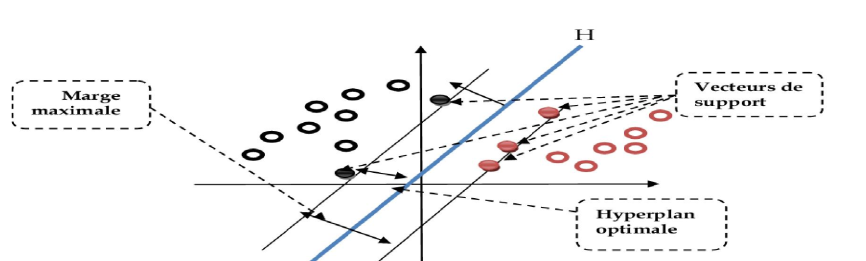
\includegraphics[width=14cm]
{images/marge.png}
\caption{Marge.\label{fig:marge}}
\end{center}
\end{figure}

super figure~\ref{fig:fig1}.

 \subsubsection{Vecteur de support}
Ce sont les points les plus proches de l’hyperplan optimal et qui déterminent la marge.

\begin{figure}[h!]
\begin{center}
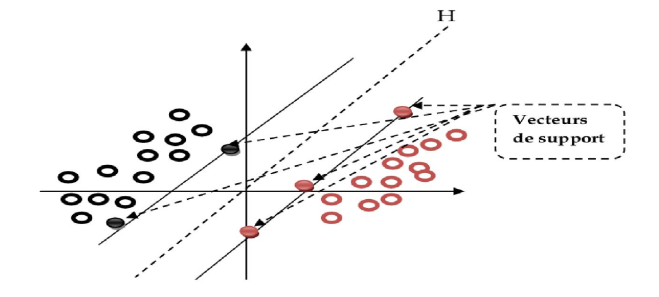
\includegraphics[width=14cm]
{images/vecteurs.png}
\caption{Vecteurs de support.\label{}}
\end{center}
\end{figure}

super figure~\ref{fig:vecteur}.

\subsection{Principe des SVM}

Comme dit précédemment, les SVMs peuvent être utilisés pour résoudre des
problèmes de classification. La résolution d'un tel problème passe par la
construction d'une fonction h définit par :
\[
  y = h(x_i) = <w, x_i> + b = \sum_{j=1}^p w_j.x_i^j + b
\]
Où $w$ est le vecteur poids et $b$ le biais.  
Pendant son entrainement , le svm calculera un hyperplan vectoriel d'équation
$w_1.x_1 + w_2.x_2 + \cdots + w_n.x_n = 0$ ainsi qu'un scalaire $b$.

Une fois l'entrainement terminé, pour classer un nouvelle exemple $x$, le SVM
regardera le signe de la fonction :
$$ h(x) = w_1a_1 + w_2a_2  \cdots +w_na_n $$
Si $h(x)$ est positif ou nul, alors $x$ est d'un côté de l'hyperplan et
appartient à la première classe de notre dataset. Sinon $x$ appartient à l'autre
classe.

En résumé, trouver la classe d'un nouvel exemple revient à réaliser
laclassification suivante.
\[
\left\{
  \begin{array}{rcr}
    <w, x_i> + b \ge 1  si y_i =1 \\
    <w, x_i> + b \le -1  si  y_i = -1 
  \end{array}
\right.
\]

Trouver l’hyperplan optimal revient à maximiser la marge M et donc à maximiser la
somme des distances euclidienne (d) des deux classes par rapport à l’hyperplan.
\subsubsection{Calcul et Maximisation de la marge}

Considérons  un point $x_k$, on montre que sa distance à l'hyperplan de vecteur
de support $w$ et de biais $b$ est donnée par 
$$
 % \frac{l_k(w^T.x_k + b)}{\|$w$\|} \] 
$$
où $\|$w$\|$ désigne la norme euclidienne de $w$. La marge d'un hyperplan de paramètre
$(w,b)$ par rapport à un ensemble de points $(x_k)$ est donc 


Maximiser la marge est un problème d'optimisation sous contrainte. Il s'agit du
problème suivant: 
$$
aaaaaa
$$
Ce genre de problème est appelé problème d’optimisation quadratique, et il
existe de nombreuses méthodes pour le résoudre. Dans le cas des SVMs la méthode
des multiplicateurs de Lagrange est utilisé.
Intuitivement, le fait d'avoir une marge plus large procure plus de sécurité lorsqu’on
classe un nouvel exemple. En 1995, le russe Vladimir Vapnik a prouvé que cete
maximisation produit un hyperplan optimal c'est-à-dire qui donnera lieu à
moins d'erreur possible.

\subsection{Recherche de l'hyperplan optimal}

Même si on peut montrer que l’hyperplan optimal est unique, il existe 
plusieurs couples $(w, b)$ qui décrivent ce même hyperplan. On décide de ne
considérer que l’unique paramétrage $(w, b)$ tel que les vecteurs support
$x_s$ vérifient $l_s (w^T \cdot x_s + b) = 1$. Par conséquent , 
$\forall k, l_k(w^T.x_k + b) \geq 1 $. L'égalité est atteinte lorsque $x_k$ est
un vecteur de support.
La normalisation sur $w$ et $b$ permet de garantir que la marge 

\subsection{Système non linéaire}

On dit que des données sont non linéairement séparables quand il n’existe pas 
d’hyperplan capable de séparer correctement les deux catégories. Ce qui, 
d’ailleurs, arrive quasiment tout le temps en pratique. L’idée est de projeter
les points d’apprentissage dans un espace d’Hilbert(esppace de redescription)
H de dimension plus élevée dans lequel les données transformées deviennent 
linéairement séparable
L’idée de cette redescription du problème est de considérer que l’espace 
actuel, appelé espace de description, est de dimension trop petite; alors que 
si on plongeait les données dans un espace de dimension supérieure, appelé 
espace de redescription, les données seraient linéairement séparables.

\subsubsection{Astuce du noyau}
 Plus on se plonge dans une grande dimension, plus les calculs sont longs. Quand
 on pose le problème d’optimisation quadratique, on s’aperçoit que les seules
 apparitions de  


